\documentclass[12pt,a4paper]{report}
\usepackage[utf8]{inputenc}
\usepackage[spanish]{babel}
\usepackage{amsmath}
\usepackage{amsfonts}
\usepackage{amssymb}
\usepackage{graphicx}
\usepackage[left=2cm,right=2cm,top=2cm,bottom=2cm]{geometry}
\usepackage{listings} %Inserta código en el archivo
\usepackage{graphicx} %Inserta imagenes en el archivo
%\usepackage{cite} % para contraer referencias
%\usepackage{lscape} %cambia la horientación de la página a horizontal
\usepackage{hyperref} %permite insertar direcciones web

%\usepackage{fullpage}


\begin{document}

\title{Plan de tesis}
\author{Villanueva Portella, Jhon Gesell}
\date{18/03/2019}
\maketitle

\section{Introducción}
%	\begin{itemize}
%	\item Importancia
%	\item Antecedentes
%	\item Justificaci\'on del m\'etodo utilizado
%	\item Valor agregado de nuestra propuesta	
%	\end{itemize}
Un paquete hidro-sedimentario ayuda a la toma de mejores decisiones en la gestión de los recursos hídricos consolidando una base de datos que permita recopilar a lo largo de los años los datos de hidráulica y de sedimentos. Esta base ayuda a poder analizar el comportamiento de los rios, determinar las épocas de máximas crecidas y secas.

Contar con una base igualmente permite tener un mejor acceso para un mayor público científico y técnico.

Una de las ventajas de tener una herramienta con paquetes libres es el acceso, la continua actualización y evitar la pirateria de software.



El paquete que se desea proponer brindará las posibilidades de acceso libre a centros de estudio y centros de investigación; la propuesta pretende beneficiar a todos ellos, con este motivo se pone bajo la licencia GPL V3 ( General Public License).
\section{Objetivos}
	\subsection{Ojetivos Generales}
	\begin{itemize}
	\item Crear un software hidrosedimentario con interfaz gráfica de usuario.
	\item Brindar un producto que ayude a los científicos e ingenieros que trabajan con fluídos geofísicos.
	\item Entregar un producto open-source para la comunidad científica internacional.
	\end{itemize}
	\subsection{Objetivos Específicos}
	\begin{itemize}
	\item Crear una lectura de archivos de caudales.
	\item Crear un formulario para insertar los datos de las muestras se sedimentos.
	\item Crear una base de datos.
	\item Gráficar la sección del río para visualizar las cotas de fondo y los valores de sedimentos en suspensión.
	\end{itemize}

\section{Hipótesis}
	El software que se desarrolla mediante la presente investigación debe ser calibrado con el software Winriver II de la empresa Teledyne Marine para la visualización de datos brindados por el ADCP (Perfilador de Corriente Acústico Doppler por sus siglas en ingles) Rio Grande de 1200 kHz y a su vez por el VMT (Velocity Mapping Toolbox) de la USGS (Servicio Geológico de los Estados Unidos por sus siglas en ingles) para así ofrecer valores cercanos al $5\%$ de este.

\section{Materiales y métodos}
\begin{enumerate}
\item Materiales
	\begin{enumerate}
	\item Datos recopilados del campo por el ADCP Rio Grande de 1200 kHz: \\
	Los datos que se encuentran almacenados en el ordenador sobre el cual se esta trabajando son llamados mediante el programa "gestor de caudales líquidos y sólidos".
	\item Datos del laboratorio ingresados por el usuario: \\
	Consiste en insertar en el software propuesto la tabla de muestras procesadas en laboratorio de muestras sólidas.
	\item Librería de desarrollo de aplicaciones con interfaz gráfica de usuario: \\
	PyQt5 es la librería de código abierto que permite trabajar en el lenguaje Python haciendo uso de multiples clases para así poder aprovechar el framework Qt5 Design.
	\item Lenguaje de programación Python: \\
	Es un lenguaje open-source multiplataforma y multipropósito que viene creciendo en diferentes campos, hoy muy usado en el campo científico, tiene una gran comunidad en todo el mundo, tiene una sintáxis fácil y limpia.
	\item SQLite3: \\
	Es un facilitador de base de datos liviano y robusto multiplataforma teniendo alcance de hasta 2 TB por cada base de datos.
	
	\end{enumerate}
\item Métodos
	\begin{enumerate}
	\item Lectura de archivos brindados por el usuario.
	\item Insertar datos por el usuario.
	\item Almacenamiento en la base de datos.
	\item Generación de una matríz.
	\item Interpolación de puntos.
	\item Gráfica de la sección del río.
	\item Gráfica de las celdas de aforo.
	\item Cálculo del caudal.
	\end{enumerate}
\end{enumerate}
\section{Resultados esperados}

\begin{enumerate}

\item Viesta preliminar de la interfaz gráfica de usuario \\
Para ello vea a la Figura~\ref{fig:Vista_preliminar_de_HyDro-Desktop}

\begin{figure}
  \centering
    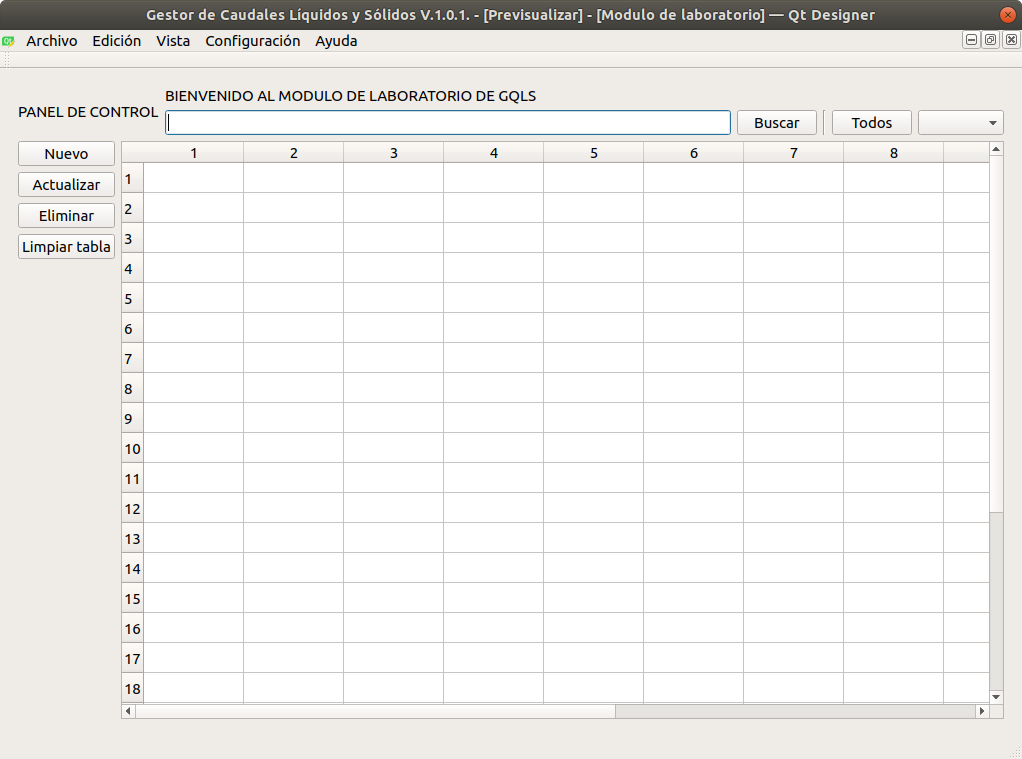
\includegraphics[width=0.7\textwidth]{imagenes/GUI_N01_V01}
  \caption{Vista construída con Qt Designer}
  \label{fig:Vista_preliminar_de_HyDro-Desktop}
\end{figure}

\item Base de datos
Se ha elaborado unos scripts que permiten crear la tabla; llenar, actualizar y eliminar los registros que constituyen la base de datos. Todo esto se logró desde el lenguaje Python3.6, los códigos se visualizan en los Anexos 01, 02 y 03 respectivamente.

Para ello vea a la Figura~\ref{fig:Vista_archivo_database_sediments}



\begin{figure}
  \centering
    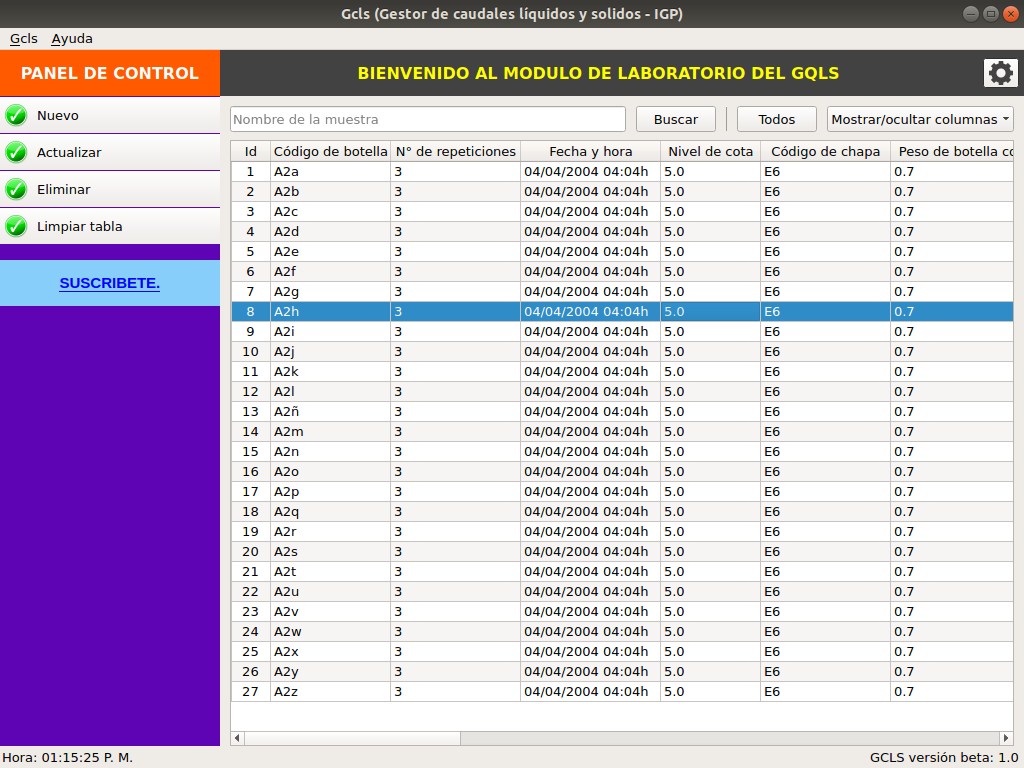
\includegraphics[width=0.7\textwidth]{imagenes/GUI_N02_V01}
  \caption{Tabla ingresada por el usuario mediante cuadros de dialogo}
  \label{fig:Vista_archivo_database_sediments}
\end{figure}


\end{enumerate}

\section{Cronograma}

\begin{center}

\begin{tabular}{|c|c|c|c|c|c|c|c|}
\hline
Meses & Junio & Julio & Agosto & Septiembre & Octubre & Noviembre & Diciembre\\ \hline
R.I. & x &  - & - & - & - & - & - \\ \hline
L.B. & x &  x & - & - & - & - & - \\ \hline
C.B.D. & x &  - & - & - & - & - & - \\ \hline
C.F. & x &  - & - & - & - & - & - \\ \hline
I.F.B.D. & - & x & - & - & - & - & - \\ \hline
I.R. & - &  - & x & x & - & - & - \\ \hline
A.M. & - &  - & - & - & x & - & - \\ \hline
C.M. & - &  - & - & - & - & x & - \\ \hline
M.U. & - &  - & - & - & - & - & x \\ \hline
\end{tabular}

\end{center}

\begin{itemize}
\item Leyenda:
	\begin{itemize}
	\item R.I.: Recolección de información.
	\item L.B.: Lectura de la bibliografía.
	\item C.B.D.:Creación de la base de datos.
	\item C.F.: Creación del formulario.
	\item I.F.B.D.: Implementación funcional de la base de datos.
	\item I.R.: Impresión de resultados en la GUI.
	\item A.M.: Ajustes del modelo.
	\item C.M.: Corrección del modelo.
	\item M.U.: Manual de usuario.
	\end{itemize}
\end{itemize}

\section{Discusiones}

\section{Conclusiones}

\section{Bibliografía}
\begin{itemize}
	\item Gonzáles, R. (s.f.). \textit{Python para todos}. Recuperado de: \textbf{http://mundogeek.net/tutorial-python}
	\item Coutinho, N. (2016). \textit{Introducción a la programación con Python: Algoritmos y lógica de programación para principiantes}, Brasil: Novatec Editora Ltda.
	\item Harwani, B. (2018). \textit{Qt5 Python GUI Programming Cookbook: Building responsive and powerful cross-platform applications with PyQt}, Estados Unidos: Packt Publishing Ltd.
	\item Owens, M. and Allen, G. (2010). \textit{The Definitive Guide to SQLite}, Estados Unidos: Springer.
	\item Johansson, R. (2015). \textit{Numerical Python}, Estados Unidos: Springer
	\item Carneiro, M. (2007). \textit{Manual de redacción superior}, Perú: Editorial San Marcos E.I.R.L.
\end{itemize}

\section{Anexos}
\subsection{Base de datos}
\begin{enumerate}
\item Creación de la tabla. \\
\textit{CrearTablaSedimentos.py}
\begin{lstlisting}
#!/usr/bin/python
# -*- coding: cp1251 -*-

# Crear base de datos y tabla con sqlite3
# 20/06/2018

__autor__ = u"Jhon Gesell"

import sqlite3

conexion = sqlite3.connect('tablasedimentos.db')
cursor = conexion.cursor()

#Crear tabla
cursor.execute('''CREATE TABLE MUESTRAS
                (CODIGO TEXT NOT NULL,
                 REPETICIONES TEXT NOT NULL,
                 FECHA TEXT NOT NULL,
                 COTA_NIVEL REAL NOT NULL,
                 COD_CHAPA TEXT NOT NULL,
                 PESO_BOTELLA_CON_LIQUIDO REAL NOT NULL,
                 PESO_BOTELLA REAL NOT NULL,
                 VOLUMEN REAL NOT NULL,
                 FINOS_PESO_INICIAL_FILTRO REAL NOT NULL,
                 FINOS_PESO_FINAL_FILTRO REAL NOT NULL,
                 GRUESOS_PESO_INICIAL_FILTRO REAL NOT NULL,
                 GRUESOS_PESO_FINAL_FILTRO REAL NOT NULL,
                 ESTACION TEXT NOT NULL)''')
conexion.close()

\end{lstlisting}

\item Insersión de registros en los campos. \\
\textit{datossedimetos.py}
\begin{lstlisting}
#!/usr/bin/python
# -*- coding: cp1252 -*-

# Insertar datos de una tabla con sqlite3
# 21/06/2018

__autor__ = u"Jhon Gesell"

import sqlite3

codigo = raw_input("Codigo: ")
repeticiones = raw_input("Repeticiones: ")
fecha = raw_input("Fecha: ")
cota_nivel = raw_input("Cota nivel: ")
cod_chapa = raw_input("Codigo de botella: ")
peso_botella_con_liquido = raw_input("Peso botella con liquido:
")
peso_botella = raw_input("Peso botella: ")
volumen = raw_input("Volumen: ")
finos_peso_inicial_filtro = raw_input("Peso inicial filtro fino:
")
finos_peso_final_filtro = raw_input("Peso final filtro fino:
")
gruesos_peso_inicial_filtro = raw_input("Peso inicial filtro
grueso:
")
gruesos_peso_final_filtro = raw_input("Peso final filtro grueso:
")
estacion = raw_input("Estacion: ")

conexion = sqlite3.connect('tablasedimentos.db')
cursor = conexion.cursor()

#Insertar datos en la tabla
cursor.execute('''INSERT INTO MUESTRAS(CODIGO, REPETICIONES,
FECHA, COTA_NIVEL, COD_CHAPA, PESO_BOTELLA_CON_LIQUIDO,
PESO_BOTELLA, VOLUMEN, FINOS_PESO_INICIAL_FILTRO,
FINOS_PESO_FINAL_FILTRO, GRUESOS_PESO_INICIAL_FILTRO, 
GRUESOS_PESO_FINAL_FILTRO, ESTACION)
                VALUES ('%s', '%s', '%s', '%s', '%s',
                '%s', '%s', '%s', '%s', '%s', '%s', '%s', '%s')
                ''' %(codigo, repeticiones, fecha, cota_nivel,
                cod_chapa, peso_botella_con_liquido,
                peso_botella,
                volumen, finos_peso_inicial_filtro,
                finos_peso_final_filtro,
                gruesos_peso_inicial_filtro,
                gruesos_peso_final_filtro, estacion))

conexion.commit()
conexion.close()
\end{lstlisting}

\item Actualización de registros en los campos. \\
\textit{ActualizarSedimentos.py}
\begin{lstlisting}
#!/usr/bin/python
#-*- coding: cp1252 -*-

# Actualizar datos en una tabla con sqlite3
# 23/06/2018

__autor__ = u"Jhon Gesell"

import sqlite3

#codigo = raw_input("Codigo: ")
#repeticiones = raw_input("Repeticiones: ")
fecha = raw_input("Fecha: ")
#cota_nivel = raw_input("Cota nivel: ")
cod_chapa = raw_input("Codigo de botella: ")
#peso_botella_con_liquido = raw_input("Peso botella con liquido:
")
#peso_botella = raw_input("Peso botella: ")
volumen = raw_input("Volumen: ")
#finos_peso_inicial_filtro = raw_input("Peso inicial filtro fino:
")
#finos_peso_final_filtro = raw_input("Peso final filtro fino:
")
#gruesos_peso_inicial_filtro = raw_input("Peso inicial filtro
grueso: ")
#gruesos_peso_final_filtro = raw_input("Peso final filtro grueso:
")
#estacion = raw_input("Estacion: ")

conexion = sqlite3.connect('tablasedimentos.db')
cursor = conexion.cursor()

#Actualizar datos en la tabla
cursor.execute("UPDATE MUESTRAS SET VOLUMEN=:volumen
WHERE FECHA=:fecha and COD_CHAPA=:cod_chapa",
                {"volumen": volumen, "fecha": fecha,
                "cod_chapa": cod_chapa})

conexion.commit()
\end{lstlisting}

\item Eliminación de registros por campos. \\
\textit{vaciartablasedimentos.py}
\begin{lstlisting}
#!/usr/bin/python
#-*- coding: cp1252 -*-

# Borrar datos en una tabla con sqlite3

__autor__ = u"Jhon Gesell"

import sqlite3

codigo = raw_input("Codigo: ")
#repeticiones = raw_input("Repeticiones: ")
#fecha = raw_input("Fecha: ")
#cota_nivel = raw_input("Cota nivel: ")
#cod_chapa = raw_input("Codigo de botella: ")
#peso_botella_con_liquido = raw_input("Peso botella con liquido:
")
#peso_botella = raw_input("Peso botella: ")
#volumen = raw_input("Volumen: ")
#finos_peso_inicial_filtro = raw_input("Peso inicial filtro fino:
")
#finos_peso_final_filtro = raw_input("Peso final filtro fino:
")
#gruesos_peso_inicial_filtro = raw_input("Peso inicial filtro
grueso: ")
#gruesos_peso_final_filtro = raw_input("Peso final filtro
grueso: ")
#estacion = raw_input("Estacion: ")

conexion = sqlite3.connect('tablasedimentos.db')
cursor = conexion.cursor()

#Eliminar datos en la tabla

cursor.execute("DELETE FROM MUESTRAS WHERE CODIGO = %s" %codigo)
conexion.commit()

conexion.close()
\end{lstlisting}


\end{enumerate}

\end{document}